% !TEX root = ../main.tex

\chapter{基于临界相变理论的早期预警特征学习与应用}
\label{chap:critical-transection}

\section{引言}

% 临界相变的普适性,早期预警特征的存在性和普遍性


% 早期预警指标的潜在原因
复杂动态系统在临近一个特定域值时将会经历临界相变\cite{ladyman2013complex},这样的临界点存在是动态系统固有的非线性和随机性导致的结果\cite{bar1997dynamics,endy2005foundations}。虽然工业系统似乎与生态系统有所不同,但类似于喷气发动机,机车和轴承这样的系统都属于动态系统,并且在复杂的内部因素和环境因素相互作用下表现出非线性和随机波动性\cite{strogatz2018nonlinear,cotilla2012predicting}。

% 工业系统面临的挑战
在工业系统中发现潜在故障极其具有挑战性。虽然系统的设计都基于定义良好的物理方程,然而系统内部组件之间和系统与工作环境之间存在复杂关系以至于很难甚至不可能穷尽所有的解析模型\cite{chan2007data},即使可以通过故障物理机制或可靠性分析来识别失效过程,但真实的工作状态和工作环境也很难完全复现。再者,生产过程的全球化成为了全面理解领域知识的阻碍,工业系统故障预测问题仍然是全球范围内的挑战。因此学习对领域知识依赖更少甚至不依赖的有效且通用的失效早期预警特征十分具有吸引力。

% 本文工作,这里要高度概括,放到设计部分。
综上所述,本文引入基于临界相变的状态分析理论,提出系统失效早期预警特征学习方法,并基于此提出关键跳变检测算法预测系统失效,此过程只需依赖少量失效敏感时间序列,可有效应对故障数据小样本、不完备特性的挑战。

\section{总体框架}
\label{sec:csd-framework}

如图\ref{fig:csd-framework},本章的总体内容结构,分为特征学习和特征应用两部分。其中特征学习包括随机波动信号挖掘、系统早期预警特征学习、系统失效与临界相变一致性检验。

(1)原生时间序列

本文基于4个来自不同系统的数据集展开研究和应用工作,这些系统包括柴油机车的制动管(气动系统),涡轮发动机(机械电子系统),IGBT(电力电子系统)和滚动轴承(机械系统)。柴油机车的制动管数据采集自本文所依托项目的商业运营机车,剩下的3个数据集是NASA预测卓越中心公开的基准数据集\cite{nasa2018}。所有的数据集都是通过传感器在系统从正常运行到失效过程中采集的单元或多元时间序列。详细介绍参见\ref{sec:csd-dataset}。

本文对数据及基于此的操作进行如下定义:以小写字母$x,y,z,...$表示时间序列。采样长度为\emph{n}的时间序列可表示为$x=\{x_{1}, x_{2}, ..., x_{n}\}$,其中$\{1,2,3,...,n\}$为下标也可看成采样时间点。$x_{t}$表示时刻$t$的观察值。$x(t)$表示从时刻\emph{t}开始到时间序列\emph{x}结尾的子序列。特别的当进行多子序列讨论时,比如对于任意整数 $i,j$ 并且$1 \leqslant  i,j \leqslant n, i \neq j$,有子序列$x(i),x(j)$,此时$x(i),x(j)$自动对齐,即较长的子序列从后往前进行截断以保证与较短子序列的长度一致,形式化的定义如下,不失一般性假设$i<j$,令$k=j-i$,那么$x(i)=\{x_{i}, ..., x_{n-k}\}, x(j) = \{x_{j}, ..., x_{n}\}$。

(2)随机波动信号挖掘

%传感器信号是以离散方式采集的时间序列,往往是一个或多个观测信号叠加的结果。
在复杂生态系统中,去趋势\cite{wang2012flickering}的操作通常用于抽取时间序列的随机波动部分以支持早期预警特征分析\cite{cotilla2012predicting}。基于时间序列的可列可加性,本文设计了随机波动信号挖掘(Fluctuation Mining, FM)框架,以保证提取的随机波动信号不存在与系统设计操作的直接关联性。首先对时间序列中的多个工作态进行识别与分离,然后通过相关性分析和/或少量专家知识识别失效敏感的工作态信号,最后通过物理方程或统计方程对操作趋势进行拟合剥离,而余下成分通过验证后则为系统固有随机波动信号。详细介绍参见\ref{sec:fluctuation-mining}。

(3) 系统失效早期预警特征学习

基于上一步挖掘的系统固有随机波动信号以及“系统失效与复杂系统临界相变一致”的假设,进行系统失效早期预警特征学习,研究早期预警特征是否可以被发现。首先基于系统的随机波动信号计算反应时间序列特性的滑动方差(Variance)、滑动自相关(Autocorrelation(1))和滑动偏斜度(Skewness);然后采用肯德尔(Kendall)趋势检验和敏感性分析进行有效性和鲁棒性进行检验。
详细介绍参见\ref{sec:csd-early-warning-mining}。
% 实验结果显示:所有系统,虽然属于不同工程系统类别,但临近失效过程中一致出现了CSD和偏斜度增加的早期预警特征,暗示了早期预警特征可作为系统失效的前兆。

(4) 系统失效与临界相变一致性检验

基于系统的原生时间序列检验假设——“系统失效与复杂系统临界相变一致”。若威尔科克森检验(Wilcoxon test)\cite{bisgaard2011time}、核密度估计\cite{bisgaard2011time}、基于赤池信息量准则(Akaike Information Criterion, AIC)的ARIMA模型分析和动态系统稳定性分析\cite{brunton2016discovering}均验证系统失效前后发生状态变迁,则证明系统失效与临界相变是一致的。详细介绍参见\ref{sec:csd-existence-test}。
% 实验结果表明被研究的系统在失效过程中确实经历了状态的突然转变,强有力的证明了工程系统失效和临界相变的一致性,进一步证明临界相变早期预警特征对系统失效预测的适用性。

(5) 系统失效(临界相变)早期预警特征应用

验证早期预警特征的存在性、有效性以及通用性之后,本文将系统失效(临界相变)早期预警特征统一称为{\heiti 系统失效早期预警特征},并将其应用到故障诊断、故障预测、状态监控和可视化展示等任务中。详细介绍参见\ref{sec:csd-application}。

\begin{figure}[H]
\centering
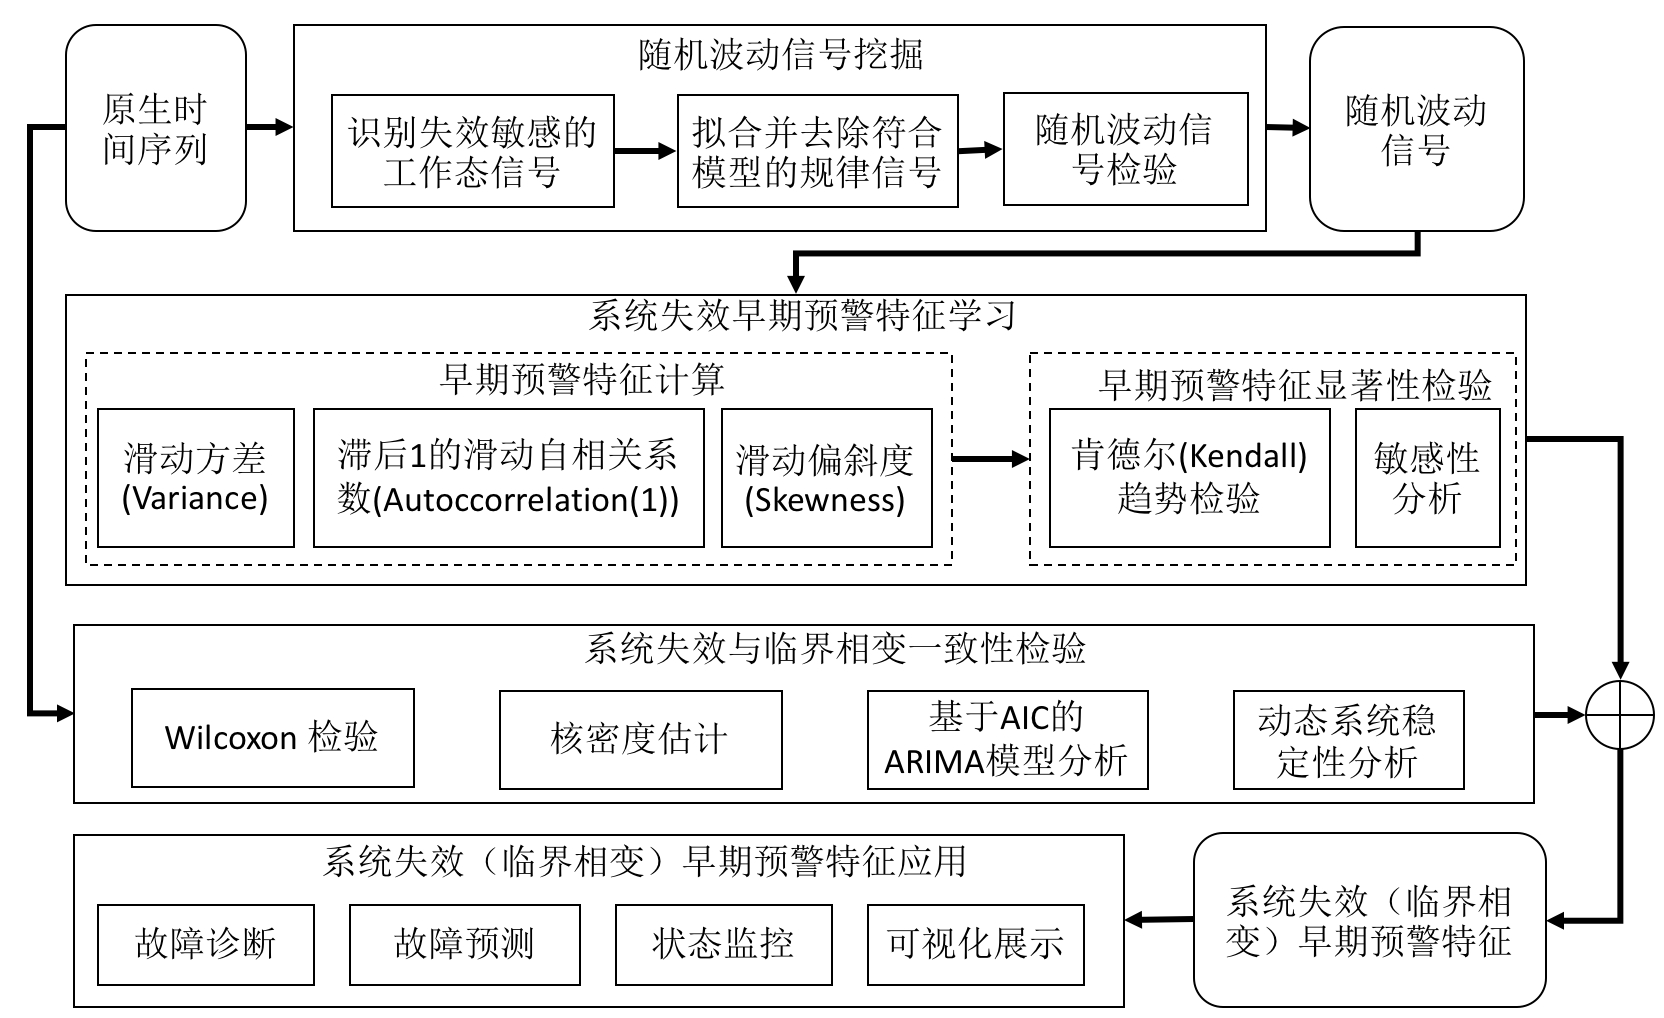
\includegraphics[scale=0.5]{csd-framework.png}
\caption{基于临界相变理论的早期预警特征学习、验证及应用的框架}
\label{fig:csd-framework}
\end{figure}

\section{系统失效早期预警特征学习}
\label{sec:csd-feature}

\subsection{随机波动信号挖掘}
\label{sec:fluctuation-mining}

通过传感器采集的时间序列常常存在多态性,即多个工作态混合(如图\ref{fig:fm-main-example}所示的信号明显存在两个工态,红色矩形标出),其中包含了对失效敏感的模式和非失效敏感的模式。基于时间序列的可列可加性,可以对时间序列进行如图\ref{fig:fm-main-structure}所示的拆分,分为符合某种或某几种模型的规律信号和受系统不确定性和环境等复杂因素影响的随机波动信号(又可称为残差)。随机波动信号挖掘具体分为以下两步:

(1)规律信号识别:规律信号的识别方法可以分为通用方法和领域相关方法。(a)通用方法基于规律信号满足某种通用方程的假设对时间序列进行拟合学习,比如多项式回归\ref{equ:fit-multiple-regression};高斯核回归\ref{equ:fit-gausian-regression},其中\emph{K}是带宽为\emph{h}的核函数,带宽\emph{h}往往是需要选择的重要参数,\emph{x}为输入,\emph{y}为输出;自回归\ref{equ:fit-autocorrelation}等。(b) 领域相关的方法,首先通过先验知识获取规律信号的运动方程,比如本文通过专家得知图\ref{fig:fm-main-example}中低态信号每个周期的运动满足等式\ref{equ:fit-real-example},然后基于此进行参数学习以拟合规律信号。通常情况下,领域相关的模型效果更好,但当先验知识缺乏时通用模型也可提供良好支持。
\begin{subequations}
\begin{align}
y_{t} &=\sum_{i=0}^{p}\alpha_{i}t^{i} \label{equ:fit-multiple-regression}\\
y_{h} &= \frac{\sum_{i=1}^{n}K_{n}(x-x_{i})y_{i}}{\sum_{i=1}^{n}K_{n}(x-x_{i})}, K_{h}(x-x_{i}) = exp(-\frac{\left \| x-x_{i} \right \|^{2}}{2\sigma^{2} }) \label{equ:fit-gausian-regression}\\
y_{t} &= AR(p) = \alpha_{0} + \alpha_{1}y_{t-1} + \alpha_{2}y_{t-2} + ... + \alpha_{p}y_{t-p} \label{equ:fit-autocorrelation}\\
y_{t} &= exp(\alpha_{1}t + \alpha_{0}) \label{equ:fit-real-example}
\end{align}
\end{subequations}
\begin{figure}[H]
\centering
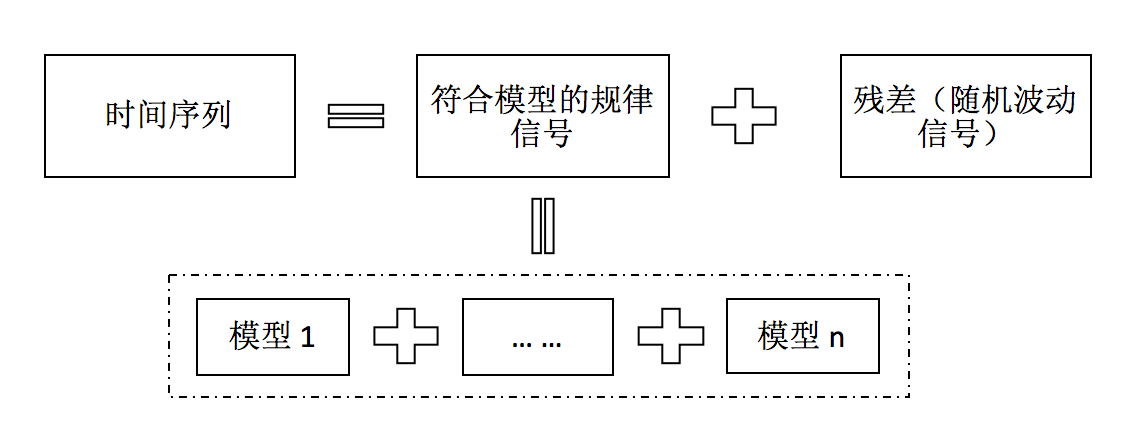
\includegraphics[scale=0.5]{fm-main-structure.png}
\caption{时间序列的可列可加性}
\label{fig:fm-main-structure}
\end{figure}
\begin{figure}[H] 
\centering
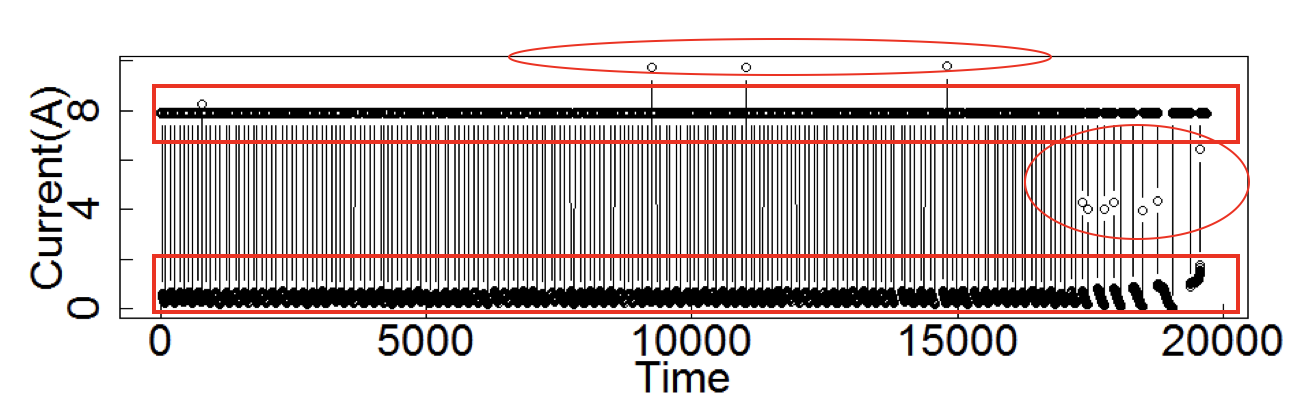
\includegraphics[scale=0.5]{fm-main-example.png}
\caption{来自 NASA IGBT 数据集的电流数据}
\label{fig:fm-main-example}
\end{figure}

(2)随机波动信号萃取:随机波动信号为原生时间序列减去规律信号而得到的残差,反应了系统受各种复杂因素影响的随机波动性,又常称为随机噪音。在异常分析或研究系统对随机波动干扰的抵抗能力时,残差信息尤为关键。 比如图 \ref{fig:fm-main-example} 为 IGBT 系统从正常到失效过程的电流信号,可以看到当系统濒临失效时噪音信号尤为密集(椭圆标出部分)。

在实际分析中明确何时使用何种信号尤为关键。本文在对系统正常情况下的运动轨迹进行建模时关注的是规律信号,参见本文章节\ref{chap:symbolic-regression};而对系统的随机波动性进行研究时,反应系统随机波动性的残差信号是关键,这将是本章的核心资源。



\subsection{系统失效早期预警特征学习}
\label{sec:csd-early-warning-mining}

\subsubsection{系统失效早期预警特征计算}

(1)关键统计量的定义:
\begin{itemize}
  \item 样本均值:定义为\ref{equ:mean},用于估计样本中心,是衡量样本集中程度的指标。
  \item 样本方差:定义为\ref{equ:var},用于估计样本偏离中心的程度,是两个样本离散程度的指标,其值越大说明样本离散程度越高。
  \item 样本协方差:定义为\ref{equ:cov},是衡量两个样本偏差的指标,若两个样本偏离其中心的方向一致则协方差为正,若两个样本偏离其中心的方向不一致则协方差为负,当协方差为零时表示总体无偏差。
  \item 自相关函数:定义为\ref{equ:acf},用于衡量时间序列与其自身滞后\emph{k}步的相关性。
  \item 自回归模型:定义为\ref{equ:ar-model},当前$x_{t}$的值与其前\emph{p}个连续时刻的值相关。$\xi$表示残差。
  \item 偏斜度:定义为\ref{equ:skew},又称样本的三阶中心矩,衡量样本分布的偏斜方向和偏斜程度。当偏斜度为零时说明样本分布以其均值为界具有完美的对称性,然而这在实际中几乎不可能发生;当偏斜度为正时说明样本分布正偏,即相对其均值往右偏离;当偏斜度为负时说明样本分布负偏,即相对其均值往左偏。偏斜度绝对值的大小衡量其偏离的程度,越大偏离程度越显著。
  \item 自相关系数:定义为\ref{equ:lag-1-autocorrelaton}。在对时间序列进行自回归分析时,距离越近相关性越强,因此普遍只通过滞后1个时刻的自相关系数来衡量时间序列与其自身的相关性,其值越大说明相关程度越高。自相关函数和自回归模型的系数都表明时间序列与其自身的相关程度,因此相关性因子可取其一,至于两者之间权衡通常根据实际情况而定。
\end{itemize}

以上的统计指标中样本方差\ref{equ:var},偏斜度\ref{equ:skew},滞后1自相关系数\ref{equ:lag-1-autocorrelaton}是计算早期预警特征的关键统计量。
\begin{subequations}
\begin{align}
& E(x) = \frac{1}{n}\sum_{i=1}^{n}x_{i} , let\ \mu (x)=E(x) \label{equ:mean}\\
& Var(x) = E((x-E(x))^{2}) = \frac{1}{n-1}\sum_{i=1}^{n}(x_{i}-E(x))^{2}, let\ \sigma(x)= \sqrt{Var(x)} \label{equ:var}\\
& Cov(x,y) = E((x-E(x))(y-E(y))) \label{equ:cov}\\
& Acf(x, k) = \frac{Cov(x(t+k), x(t))}{\sigma(x(t+k))\sigma(x(t))} \label{equ:acf} \\
& x_{t} = Ar(x,p) = \alpha_{1}x_{t-1} + \alpha_{2}x_{t-2} + ... + \alpha_{p}x_{t-p} +\xi _{t} \label{equ:ar-model} \\
& Skew(x) = E((\frac{x-\mu(x)}{\sigma(x)})^3) \label{equ:skew} \\[0.1cm]
& Autocorrelation(x) = \left\{\begin{array}{l}
Acf(x, 1)\\ [0.1cm]
\mbox{or}\\[0.1cm]
Ar(x, 1)\\[0.1cm]
\end{array}\right. \label{equ:lag-1-autocorrelaton}
\end{align}
\end{subequations}

% 介绍滑窗的计算方法
(2)以滑窗的形式计算早期预警特征:

首先通过滑窗的形式获取不同时刻对应的固定窗口大小的时间子序列集合。如图\ref{fig:csd-main-sliding-window}所示,坐标轴上每个点对应一个时刻,令滑窗大小\emph{w}为15,自左往右沿着时间轴的方向以1个时刻为步长移动滑窗,每个滑窗对应的连续时间段对应一个子序列。每个滑窗对应的子序列反应了系统在窗口内最后一个时刻的特性。其中滑窗的大小\emph{w}为重要参数,窗口过小有可能引入过多局部细节以至于很难形成对全局临界点的趋势预测指标;而窗口过大有可能掩盖局部重要特征。通过以上操作可以获取子序列集,定义为\ref{equ:rolling-set}。值得注意的是由于窗口大小的限制,前$w-1$个时刻没有对应的子序列,这部分信息将被丢弃,若采样点足够或前期采样点可视为不稳定采样点那么丢弃此部分信息带来的影响可以忽略,但仍需注意窗口设置过大可能导致关键信息丢失的问题。

在获取滑窗时间序列集合后,计算滑动方差\ref{equ:rolling-var},滑动偏斜度\ref{equ:rolling-skew},滑动自相关系数\ref{equ:rolling-autocorrelation}作为早期预警特征。这些基于滑窗计算的特征具有反应系统状态的能力。比如计算滑动方差\ref{equ:rolling-var},$rolling\_var(x)=Var(rolling\_set(x))=\{Var(\{x_{i-w+1,x_{i-w}, ..., x_{i}}\}), ..., Var(\{x_{n-w+1,x_{n-w}, ..., x_{n}}\})\}=\{v_{w}, ..., v_{n}\}$,其中$v_{i}, i=w,w+1,...,n$反应系统在时刻\emph{i}的状态特性。
\begin{subequations}
\begin{align}
& rolling\_set(x) = \{\{x_{i-w+1}, x_{i-w}, ..., x_{i}\} | i=w, w+1, ..., n\} \label{equ:rolling-set} \\[0.1cm]
& rolling\_var(x) = Var(rolling\_set(x)) \label{equ:rolling-var} \\[0.1cm]
& rolling\_skew(x) = Skew(rolling\_set(x)) \label{equ:rolling-skew} \\[0.1cm]
& rolling\_autocorrelation(x) = Autocorrelation(rolling\_set(x)) \label{equ:rolling-autocorrelation}
\end{align}
\end{subequations}

\begin{figure}[H]
\centering
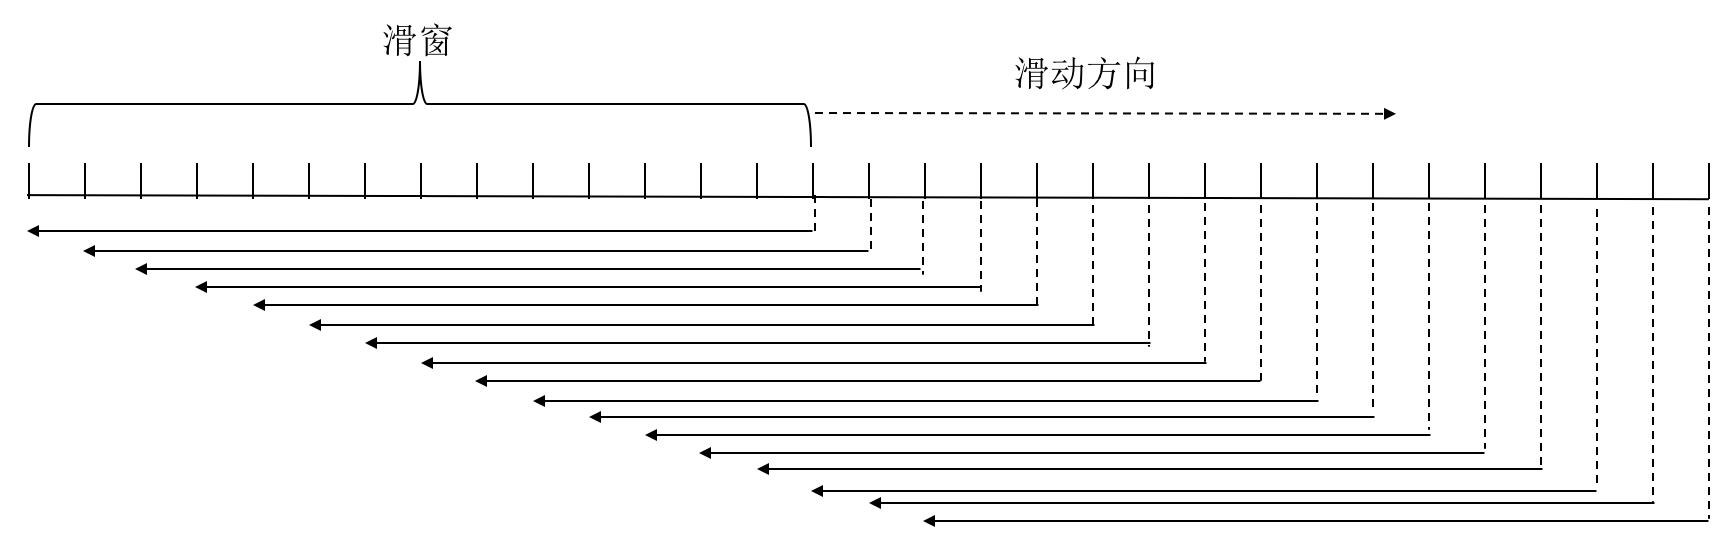
\includegraphics[scale=0.5]{figures/csd-main-sliding-window.png}
\caption{滑窗获取不同时刻时间子序列构成的集合}
\label{fig:csd-main-sliding-window}
\end{figure}

\subsubsection{系统失效早期预警特征显著性检验}

早期预警特征在稳定状态下没有显著波动,当临近系统失效时出现明显的趋势特征,此特征可作为预测指标。本文采用Kendall趋势检验和敏感性分析分别检验早期预警特征的有效性和鲁棒性。

(1)基于Kendall的早期预警特征趋势显著性检验

% 趋势显著性度量
% What is the Mann Kendall Trend Test?: http://www.statisticshowto.com/mann-kendall-trend-test/
% R 的文档“Non-Parametric Trend Tests and Change-Point Detection”,有精确的定义:https://cran.r-project.org/web/packages/trend/vignettes/trend.pdf
% R 的实现文档,更清楚的描述了流程:https://vsp.pnnl.gov/help/vsample/Design_Trend_Mann_Kendall.htm
% 百度百科给出了 Mann Kendall 的优势:https://baike.baidu.com/item/Mann-Kendall%E8%B6%8B%E5%8A%BF%E6%A3%80%E9%AA%8C%E6%B3%95/17829790
Kendall趋势检验为非参数统计检验方法,一般用于检验序列是否存在明显的单调趋势。Kendall趋势检验因具有以下优势得到广泛应用(a)被检验序列无需满足任何先验分布假设,即使存在极端值也可以进行检验;(b)允许被检验序列存在缺失值;(c)检验过程主要分析相对数量级而非数值本身,因此被检验序列可以是微量值;(d)不局限于线性趋势。

Kendall趋势检验的原假设$H_{0}$为“数据来源于相互独立且同分布的总体”,相应的备择假设$H_{A}$为“数据存在单调趋势”。具体检验过程可分为以下几步:

1.计算秩和统计量。通过等式\ref{equ:kendall-s},计算$n(n-1)/2$种可能组合的差并取其符号求和得到\emph{S},其中取符号操作定义为等式\ref{equ:kendall-sgn}。

2.计算\emph{S}的方差。\emph{S}的方差由等式\ref{equ:kendal-sigma}定义,其中\emph{p}表示联结组(由相同数值组成的集合并且元素个数大于1)个数, $t_{j}$ 表示对应的联结组的元素个数。比如对于序列$\{23, 24, 29, 6, 29, 24, 24, 29, 23\}$,联结组个数$p=3$,分别为$\{23, 23\}, \{24, 24, 24\}, \{29, 29, 29\}$并依次从1开始编号,那么可得$t_{1}=2, t_{2}=3, t_{3}=3$。
%值得一提的是\emph{S}的期望为0,即$E(S)=0$。

3.计算趋势度量统计指标。通过\ref{equ:kendall-z-transformation}计算Kendall趋势检验的统计量\emph{Z},正的或负的\emph{Z}值表示序列存在上升或下降的趋势。实践中通常采用由等式\ref{equ:kendall-tau}定义的Kendall's tau 统计量来度量被测序列的趋势,其中\emph{D}定义为\ref{equ:kendall-d}。Kendall's tau 取值区间为[-1,1],当其值为0时表示序列中不存在趋势,否则正数或负数分别表明序列存在上升或下降趋势,其绝对值越大说明趋势越明显。
%本文主要采用 Kendall's tau 作为趋势显著性指标。
\begin{subequations}
\begin{align}
& S = \sum_{k=1}^{n-1} \sum_{j=k+1}^{n} sgn(X_{j} - X_{k}) \label{equ:kendall-s} \\[0.1cm]
& sgn(x) = \left\{\begin{matrix}
 1 & if & x>0 \\ 
 0 & if  & x=0 \\ 
 -1 &  if &{} x<0
\end{matrix}\right. \label{equ:kendall-sgn} \\[0.1cm]
& \sigma^{2} = \frac{n(n-1)(2n+5)-\sum_{j=1}^{p}t_{j}(t_{j}-1)(2t_{j}+5)}{18} \label{equ:kendal-sigma} \\[0.1cm]
& Z = \left\{\begin{matrix}
\frac{S-1}{\sigma} & if  & S>0 \\ 
 0 & if & S = 0\\ 
 \frac{S+1}{\sigma}& if  &  S>0
\end{matrix}\right. \label{equ:kendall-z-transformation}\\[0.1cm]
& \tau = \frac{S}{D} \label{equ:kendall-tau} \\[0.1cm]
& D=[\frac{1}{2}n(n-1)-\frac{1}{2}\sum_{j=1}^{p}t_{j}(t_{j}-1)]^{1/2}[\frac{1}{2}n(n-1)]^{1/2} \label{equ:kendall-d}
\end{align}
\end{subequations}

(2)早期预警特征的敏感性分析
% 之前论文中 method 部分总结的内容。

敏感性分析是检验早期预警特征对不同关键参数的鲁棒性。影响早期预警特征学习结果的关键因素有:随机波动信号挖掘过程采用的时间序列分解方法和滑窗大小。本文对不同参数组合进行大量重复实验,即采用不同窗口大小、不同时间序列分解方法进行早期预警特征学习,并通过Kendall趋势显著性度量各种情况下早期预警特征趋势的显著性,由此观察早期预警特征对参数的敏感性。

\subsection{系统失效与临界相变的一致性检验}
\label{sec:csd-existence-test}

本文基于原生时间序列,通过Wilcoxon符号秩检验、核密度估计、基于AIC的ARIMA分析和动态系统稳定性分析方法进行系统失效与临界相变一致性检验。

(1)Wilcoxon 符号秩检验

由于时间序列通常具有很强的自相关性并且隐含分布不明,因此本文采用非参数统计检验方法Wilcoxon来检验两个样本是否来自同一分布,其判断依据是考察两个样本是否有相同的均值。

假设从系统正常到失效过程采集的时间序列为\emph{x},从序列的正常状态取长度为\emph{w}的子序列$x\_stable = \{x_{i}, x_{i+1}, ..., x_{i+w-1}\}$,并以大小为\emph{w}的滑窗沿失效方向滑动以获取子序列集合$rolling\_set =\{\{x_{j-w+1}, x_{j-w},..., x_{j}\} | j=i+w,...,n\}$。然后检验每个滑窗子序列$x\_rolling \in rolling\_set$是否与$x\_stable$同分布,原假设$H_{0}$为“$x\_stable$和$x\_rolling$来源于同一分布”。

为了作出“接受”或“拒绝”$H_{0}$的决定,本文采用 \emph{p} 值法(又称临界值法)来对假设检验的显著水平进行度量。\emph{p}值是由检验统计量的样本观察值得出的原假设可被拒绝的最小显著性水平。\emph{p}的取值区间为$[0, 1]$,表示拒绝原假设的依据强度,\emph{p}值越小,拒绝原假设的依据越强。一般的,若$p \leqslant 0.01$则称拒绝$H_{0}$的依据很强或称检验是高度显著的;若$0.01 < p \leqslant 0.05$则称拒绝$H_{0}$的依据强或称检验是显著的;$0.05 < p \leqslant 0.1$称拒绝$H_{0}$的理由是弱的,检验不显著;若$p>0.1$一般来说没有理由拒绝$H_{0}$。

每个滑窗子序列$x\_rolling$对应一个\emph{p}值,表示拒绝$H_{0}$的强度,当\emph{p}值小到一定程度时则可有足够依据做出拒绝$H_{0}$的决定,即认为$x\_rolling$和$x\_stable$不同分布,若在系统失效时刻附近\emph{p}值急剧下降到很小的值,则有足够信心拒绝$H_{0}$,即认为此时$x\_rolling$与$x\_stable$不同分布,进而说明系统失效引起了系统状态的急剧改变。

% 核密度估计
(2)核密度估计

在统计领域,核密度估计是一种估计随机变量的概率密度函数的非参数化方法,并且基于高斯核的概率密度估计最为常用。假设从系统正常到失效过程采集的时间序列为\emph{x},将\emph{x}划分为以下3个不相交区间,$x\_stable1=\{x_{i},x_{i+1}...,x_{j}\}$、$x\_stable2=\{x_{k},x_{k+1},...,x_{l}\}$、$x\_failed=\{x_{a},x_{a+1},...,x_{b}\}, 1 \leqslant i,j,k,l,a,b \leqslant n$,分别对应系统的正常状态、正常状态和失效状态。然后通过基于高斯核的概率密度估计方法分别对$x\_stable1, x\_stable2,x\_failed$进行概率密度估计,并对概率密度函数进行可视化比较。若$x\_stable1, x\_stable2$概率密度函数基本一致,而$x\_failed$与前两者有显著不同,这就说明他们所处的状态不同,进而说明系统失效引起了系统状态的转变。

% AIC的ARIMA模型分析
(3)基于AIC的ARIMA模型分析

自相关(AutoRegressive AR)模型定义为\ref{equ:ar},表示当前时刻的观测值$z_{t}$与其自身滞后的\emph{p}个时刻的观察值相关。滑动平均(Moving Average, MA)模型定义为\ref{equ:ma},对于随机游走序列\emph{a},其当前值$a_{t}$可由其相邻的前\emph{p}个时刻的值通过加权平均来估计。自回归滑动平均模型(Autoregressive Moving Average Model, ARMA)定义为\ref{equ:arma},是自相关模型和滑动平均模型的融合。值得注意的是,以上模型的应用需要依赖时间序列稳定性假设,即时间序列中任意两个子序列的联合概率保持不变。但严格意义的稳定性在现实中很难得到满足,因此通常只需要满足弱稳定性假设,即任意子序列的均值和方差保持一致。当弱稳定性假设不能满足时可以通过微分的操作来稳定化原序列,即先通过等式\ref{equ:diff}将原序列进行稳定化后再进行ARMA分析,这通常称为自回归积分滑动平均模型(Autoregressive Integrated Moving Average Model, ARIMA),可表示为$ARIMA(p,d,q)$,$p$表示自相关滞后时长,$d$表示微分阶数,$q$表示滑动平均滞后时长。对于ARIMA模型的评估,有赤池信息量准则(AIC),基于Akaike’s偏差修正的信息准则(Akaike’s bias-corrected information criterion, AICC)和贝叶斯信息准则(Bayesian information criterion, BIC),本文采用AIC。

本文首先通过基于AIC的ARIMA模型对系统失效前的正常状态下对应的时间序列进行拟合学习,由此得到正常状态下的ARIMA模型,然后用此模型来预测未来一个时间段的观测值,预测区间包括失效状态对应的区段。理论上说,如果失效没有引起系统状态转变,正常状态下学习的模型可以对失效状态进行很好的预测,反之则说明失效状态和正常状态不同,进而说明系统失效引起了系统状态的转变。
\begin{subequations}
\begin{align}
& z_{t}=AR(p) = \alpha_{1}z_{t-1} + \alpha_{2}z_{t-2} + ... + \alpha_{p}z_{t-p} + \xi _{t} \label{equ:ar} \\[0.1cm]
& a_{t}=MA(q) = - \theta_{1}a_{t-1} - \theta_{2}a_{t-2} - ... - \theta_{q}a_{t-q} \label{equ:ma}\\[0.1cm]
& y_{t}=ARMA(p, q) =z_{t} + a_{t} = AR(p) + MA(q) \label{equ:arma} \\[0.1cm]
& Diff(d) = z_{t} - z_{t-d} \label{equ:diff} 
\end{align}
\end{subequations}

% 相空间和分叉点分析(Phase-space and Bifurcation analysis)
(4)动态系统的稳定性分析

正常的动态系统具有稳定性,在运行过程中始终向吸引子(Attractor)收敛,即使受到轻微扰动也能很快恢复到稳定状态。如图\ref{fig:csd-early-warning-signal}所示,系统在稳定状态下具有高恢复率,此时盆地的吸引力较大可以抵抗轻微扰动干扰,系统维持在吸引盆中运动;而当系统临近临界相变点时盆地的吸引力变小,相当于吸引盆变浅,此时即使轻微扰动也能将系统推出吸引盆,进而产生急剧的状态变化。

以单变量的时间序列为例,如图\ref{fig:csd-phase-plot-single-variable},纵坐标表示观测序列\emph{x}的一阶微分,反应\emph{x}的运动趋势;横坐标为\emph{x},反应其当前的运动状态。通过解$\frac{dx}{dt}=0$可以得到两个固定点,即图中的点\emph{D}和点\emph{S}。\emph{D}的稳定性分析考察如下:一方面,区间[0,D]的微分为负数,说明\emph{x}在此区间减小,即处于点\emph{D}左下邻域内的运动点有远离\emph{D}的趋势;另一方面,在[D,S]区间内,微分为正,说明\emph{x}在此区间增大,即处于\emph{D}右上邻域内的运动点有远离\emph{D}的趋势;综合两方面,固定点\emph{D}两侧的运动方向背离无法收敛于\emph{D},因此动态系统此时处于不稳定状态。点\emph{S}的稳定性考察如下:一方面,[D,S]区间对应的微分为正,说明\emph{x}在此区间增大,即处于\emph{S}左上邻域内的运动点正在靠近\emph{S};另一方面,[S,inf]对应的微分为负,说明\emph{x}在此区间减小,即处于\emph{S}右下方邻域内的运动点正在靠近\emph{S};综合两方面,固定点\emph{S}邻域的运动都收敛到点\emph{S},即点\emph{S}处于稳定状态。
\begin{figure}[H]
\centering
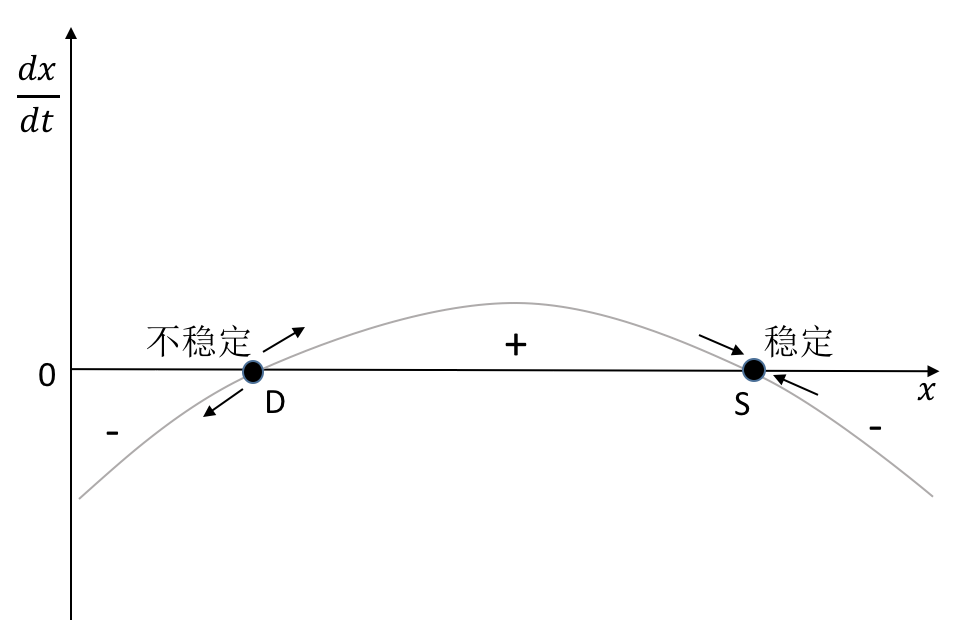
\includegraphics[scale=0.5]{figures/csd-phase-plot-single-variable.png}
\caption{一维离散采样的时间序列相空间图}
\label{fig:csd-phase-plot-single-variable}
\end{figure}
相空间(phase space)分析和分叉点(bifircation)分析常用于动态系统稳定性分析。其中分叉点分析需要知道明确的系统动态方程和分叉因子,难点在于分叉因子依赖很强的领域知识,即使动态方程可以由数据构建也很难在公式中确定分叉因子。因此本文主要采用相空间分析的方法对动态系统的稳定性进行考察。

动态系统可以分为连续型和离散型系统。主要分析流程为,本文首先尝试通过第\ref{chap:symbolic-regression}章介绍的符号回归方法对系统方程(吸引子)或微分方程进行学习。若符号回归方法可以学习有效的系统方程,本文将对应的系统视为连续型系统,并基于系统方程展开稳定性分析。否则,本文将对应的系统视为离散型系统,然后将采集的离散时间序列映射到2或3维、甚至更高维的相空间中以观察动态系统的运动轨迹和状态变化。基于以上分析作出系统是否处于稳定状态的判断。

1. 连续型系统的稳定性分析

根据变量个数的不同进行以下稳定性分析:
\begin{enumerate}[a.]
  \item 单变量模型分析。首先通过符号回归方法学习一维非线性动态方程(微分方程)$\frac{dx}{dt} = f(x)$,然后通过解方程$f(x_{0})=0$得到固定点$x_{0}$,若固定点$x_{0}$满足等式$\frac{\partial f(x)}{\partial x} | x=x_{0} < 0$,则这一点为吸引盆即稳定点。
  \item 多变量模型分析。本文通过符号回归方法学习吸引子的动态性,即多变量之间的关系,基于此本文可以观察系统的运动轨迹。若系统随时间运动过程中维持在吸引子附近,则说明系统的运动是稳定的,其中吸引子的类型有不动点、有限数量的点、有限环、有限环面、奇异吸引子等。若动态系统在运动过程中表现推斥极(repelloer)即向吸引子相反的方向运动,则说明系统处于不稳定状态。
\end{enumerate}
% \begin{subequations}
% \begin{align}
% & \frac{dx}{dt} = f(x) \label{equ:stability-one-dim-dynamic} \\[0.1cm]
% & f(x_{0}) = 0 \label{equ:stability-balance} \\[0.1cm]
% & \frac{\partial f(x)}{\partial x} | x=x_{0} < 0 \label{equ:stability-threshold}
% \end{align}
% \end{subequations}

2. 离散型系统的稳定性分析

离散型系统的状态将满足等式$x_{t+1} = f(x_{t})$,本文不直接对其进行学习,而是基于离散时间序列绘制逻辑斯谛映射图来观察动态系统的轨迹。逻辑斯谛映射图通过绘制 $x_{t+1}$ 对 $x_{t}$ 的二维相空间来反应系统的运动轨迹。以此类推,可以将序列映射到3维甚至更高维的相空间中来观察动态系统更深层的运动规律。最后通过观察系统轨迹是否表现收敛性或吸引子性质来分析当前系统是否处于稳态。
% \begin{equation}
% \label{equ:discrete-ystem}
% x_{t+1} = f(x_{t})
% \end{equation}

\section{系统失效早期预警特征应用}
\label{sec:csd-application}

系统失效早期预警特征直接反映了动态系统随时间变迁的健康状态,可直接通过用户接口进行展示,可以提供给其他机器接口实现状态检测。本节主要介绍针对早期预警特征提出的关键跳变检测算法,由此实现故障预测。

本文以 Wilcoxon 符号秩检验非参数化方法作为关键跳变检测算法设计的基础,主要原因有:(a)早期预警特征在正常状态时保持平稳,当临近系统失效时出现显著趋势,通过假设检验方法可以定位临界点;(b)时间序列分布不明,非参数化方法无需依赖先验分布。
% 介绍假设检验原理,(“临界点”)——「概率论课本180」,可以把书引进来。

核心思想为,在显著水平$\alpha$下,检验假设\ref{csd-ap-hypothesis},其中$H_{0}$为原假设;$H_{1}$为备择假设,假设检验需基于样本作出接受$H_{0}$与$H_{1}$其一的决策。
\begin{equation}
\label{csd-ap-hypothesis}
H_{0}: \mu = \mu_{0}, H_{1}:\mu \neq \mu_{0}
\end{equation}

系统失效早期预警特征在正常状态时保持平稳,因此系统处于正常状态时,早期预警特征的均值保持常数$\mu_{0}$,即接受$H_{0}$;当系统临近失效时,早期预警特征出现偏离正常均值$\mu_{0}$的上升或下降趋势,当偏离足够显著时则可作出拒绝$H_{0}$并接受$H_{1}$的决策,此边界点通常称为{\heiti 临界点},由样本和显著水平$\alpha$同时决定。$\alpha$控制范第I类错误的概率,第I类错误表示假设$H_{0}$实际上为真却被错误的拒绝。

本文有3个指标共同构成系统失效早期预警特征,令长度为$N$的时间序列\emph{x}表示其中任意一个指标。有大小为\emph{W}的滑窗,令$x(1) = \{x_{1}, x_{2}, ..., x_{W}\}$并且其均值为$\mu_{0}$,对应系统初始的稳定状态;以滑窗\emph{W}沿系统失效方向滑动,令$x(i) = \{x_{i-W+1}, x_{i-W}, ..., x_{i}\}, i=W+1,...,N$,其均值为$\mu_{i}$,对应系统在$i$时刻的状态。对$x(1)$和$x(i)$进行Wilcoxon 符号秩检验,并且原假设为$H_{0}: \mu_{0}=\mu_{i}$,$x(1)$表示系统正常状态,若某一时刻在显著水平$\alpha$下$H_{0}$被拒绝,则此刻对应临界点,同时也是预测故障的跳变点。

% reference: 
% https://en.wikipedia.org/wiki/Wilcoxon_signed-rank_test#cite_note-lowry-1
% http://www.r-tutor.com/elementary-statistics/non-parametric-methods/wilcoxon-signed-rank-test
令$xs = x(1), xr=x(i)$,针对单指标变量的 Wilcoxon 符号秩检验的流程如下:
\begin{enumerate}[1.]
  \item 对于$i=1,...,W$,计算$|xs_{i}-xr_{i}|$和$sgn(xs_{i}-xr_{i})$,其中$sgn$表示取符号操作。
  \item 称$(xs_{i}, xr_{i}), i=1,..,W$为一对样本,若$|xs_{i}-xr_{i}|=0$则成对去掉,并令$M$表示剩余样本对数。
  \item 基于$|xs_{i}-xr_{i}|$的大小,对余下的$M$对样本从小到大进行排序。
  \item 获取样本对的秩,即将排序好的样本从1开始进行排名,排名相同的样本对秩为排名均值,令$r_{i}, i=1,...,M$表示样本对$i$的秩。
  \item 计算秩和统计量$R=\sum_{i=1}^{M}[sgn(xs_{i} - xr_{i})*r_{i}]$。
  \item 在原假设,即$H_{0}$假设下,$R$服从均值为0,方差为$\frac{M(M+1)(2M+1)}{6}$的没有表达式的特定分布。若$|R| > R_{C}(\frac{\alpha}{2})$则拒绝原假设,其中$R_{C}(\frac{\alpha}{2})$是临界点。
\end{enumerate}

针对滑动方差、滑动自相关系数、滑动偏斜度3个指标分别执行以上1~5步可以得到各自的秩和统计量,分别表示为$R_{v}, R_{a}, R_{s}$,然后通过等式$U=\frac{R_{v} + R_{a} + R_{s}}{3}$计算融合统计量$U$。同理,在原假设下,$U$服从均值为0的分布,若$|U| > U_{C}(\frac{\alpha}{2})$则拒绝原假设,而第一次使拒绝原假设决策成立的时刻是预测系统失效的跳变点。

\section{实验结果及分析}
\label{sec:csd-experiment}

\subsection{数据集说明}
\label{sec:csd-dataset}	

(1) 机车空气制动器系统数据集

数据集为正在运营的商业机车2016年5月5日到15日的运行数据,数据包括制动管和制动缸的空气压力信号,在此期间空气制动管部分失效。数据通过火车控制和管理系统以1Hz的采样率采集。数据集为列车处于运行状态和停车状态下的观测数据。基于信号与失效相关性分析,本文选用运行时数据作为临界相变早期预警特征学习框架的输入。数据采集环境如图\ref{fig:sr-data-collect}。

(2) 轴承数据集

数据集来源于NASA预测卓越中心的预测数据库\cite{nasa2018}。数据由辛辛那提大学的智能维护系统中心采集,包含三个实验结果集。本文选择第二个实验结果集作为数据源,其中包含从四个轴承中采集的四个传感器信号集。来自轴承1的传感器数据是轴承从正常到失效的振动信号,最后外环失效导致系统停止运行。

(3) 涡扇发动机退化模拟数据集

数据集来源于NASA预测卓越中心的预测数据库\cite{nasa2018}。数据集产生于一个工业增强模拟器C-MAPSS。数据集包含100个仿真单元,每个单元对包含一组独立的测试到失效的过程数据。本文随机选取一组仿真单元数据作为早期预警特征学习的数据源,编号为FD001。这个数据集包含26个信号,为了方便将其表示为V1,V2,...,V26,其中V1是测试单元编号,V2是时间戳,V3-V5是操作配置信号,V6-V26是传感器观测值。在每次试验中,即采集每个单元的测试到失效过程数据时,引擎正常启动并正常运行,然后随机选取一个时刻向系统注入可引起失效的压力以引发系统失效。
%https://www.grc. nasa.gov/WWW/cdtb/software/mapss.html

(4) IGBT加速老化试验数据集

数据集来源于NASA预测卓越中心的预测数据库\cite{nasa2018}。数据集包含来自6个设备的老化数据,其中有一个设备为DC门偏差老化,其余剩下的设备为方信号门偏差老化。本文选择热负荷老化实验采集的子集,实验中通过门电压的DC偏差触发设备老化。感知的信号集包括集电极电流、集电极电压、门电流、门电压、散热器温度和包装温度。在此次加速正常到失效的老化实验中,系统在最后由于闩锁失效。在关闸阶段的集电极电流通常被认为是系统失效的指示信号。本文分析集电极电流、集电极压力和门电流来捕捉信号内和信号间的特性。
% 系统在最后由于闩锁效应(latch-up)失效
% 在关闸(switch-off)阶段

\subsection{实验结果与分析}
% 不同系统中的临界相变早期预警指标
% 说明实验的环境和参数。

实验硬件的主要参数:CPU,Intel(R) Xeon(R) CPU E5-2682,16核,2.50GHz;内存,235GB。所有算法均使用 R3.3.0 实现,若没有特殊说明,所有滑窗计算的窗口大小均为时间序列长度的一半。

(1)系统失效早期预警特征学习的结果展示

针对 4 个不同类型的数据集,分别通过本章\ref{sec:csd-early-warning-mining}描述的早期预警特征学习方法获得滑动方差(Variance)、滑动自相关系数(Autocorrelation(1))和滑动偏斜度(Skewness),并进行显著性和鲁棒性检验。图\ref{fig:csd-early-signal}是机车空气制动器系统数据集、轴承数据集、涡扇发动机退化模拟数据集和IGBT加速老化试验数据集的结果,对应的趋势指标参见表\ref{tab:csd-kd-trend}。结果表明,虽然4类系统差异很大,但临近失效时早期预警特征出现了一致且显著的上升或下降趋势,证明了本文方法的有效性和通用性。

(2)FM框架对早期预警特征的增强效果展示

如图\ref{fig:csd-fm-procedure}所示,本文以IGBT加速老化试验数据集为例展示FM的有效性,具体如下:

1.通过相关性分析发现失效敏感的低工作态信号\emph{x},对应图\ref{fig:csd-fm-procedure}a有颜色圈;

2.通过专家得知\emph{x}正常工作时遵循指数衰减的公式\ref{equ:fit-real-example},进而通过回归方法学习方程的参数,对信号轨迹的拟合效果对应图\ref{fig:csd-fm-procedure}b实线,此部分信号记为\emph{r};

3.计算随机波动信号$s = x - r$,如图\ref{fig:csd-fm-procedure}c所示。

4.基于\emph{s}计算早期预警特征,如图\ref{fig:csd-fm-procedure}f,g,h。

Variance、Autocorrelation(1)、Skewness 三个指标的原趋势分别为0.38、0.86、0.48,参见图\ref{fig:csd-early-signal}和表\ref{tab:csd-kd-trend};经过FM框架处理后的早期特征趋势分别为0.88、0.90、0.88,增强效果显著,充分证明FM框架的有效性。

\begin{figure}[H]
\centering
\begin{subfigure}{\textwidth}
    \centering
    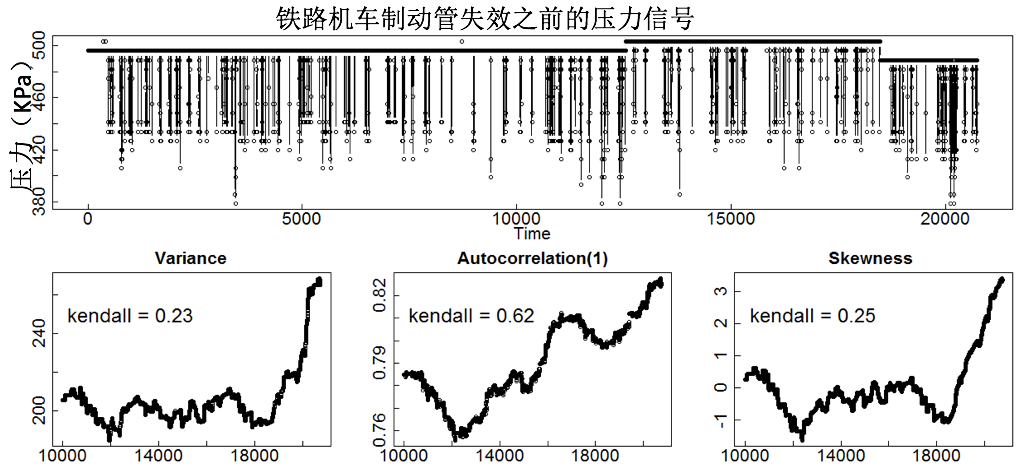
\includegraphics[scale=0.6]{figures/csd/csd-signal-locomotive.png}
\end{subfigure}\\
\begin{subfigure}{\textwidth}
  \centering
  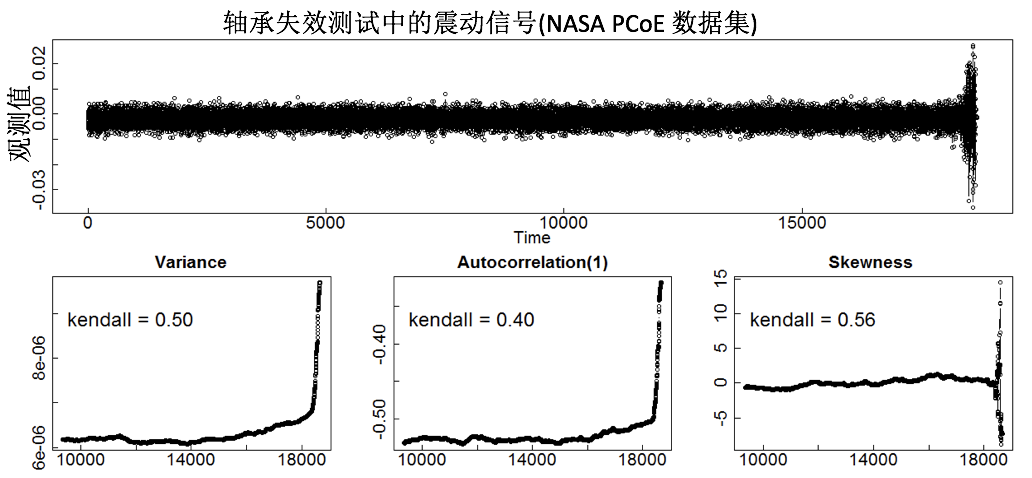
\includegraphics[scale=0.6]{figures/csd/csd-signal-bearing.png}
\end{subfigure}\\
\begin{subfigure}{\textwidth}
    \centering
    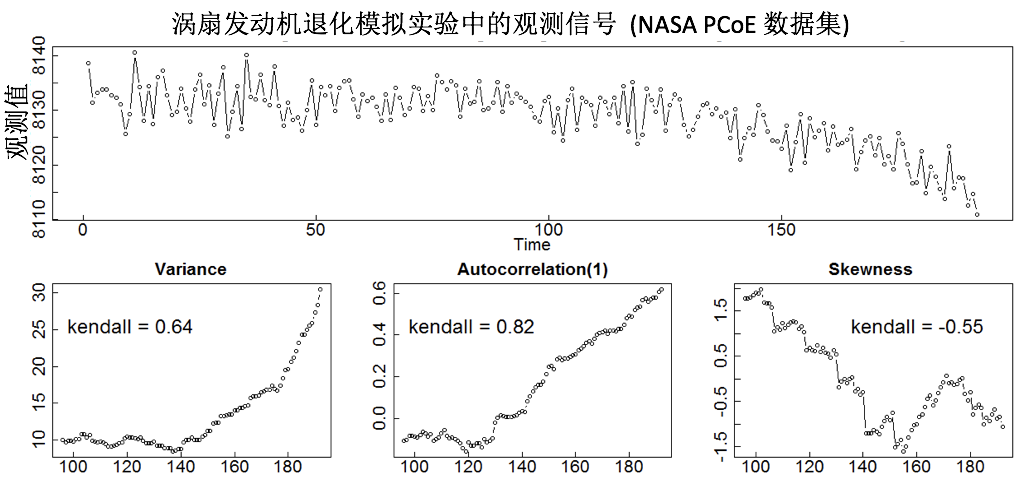
\includegraphics[scale=0.6]{figures/csd/csd-signal-turbofan.png}
\end{subfigure}\\
\begin{subfigure}{\textwidth}
    \centering
    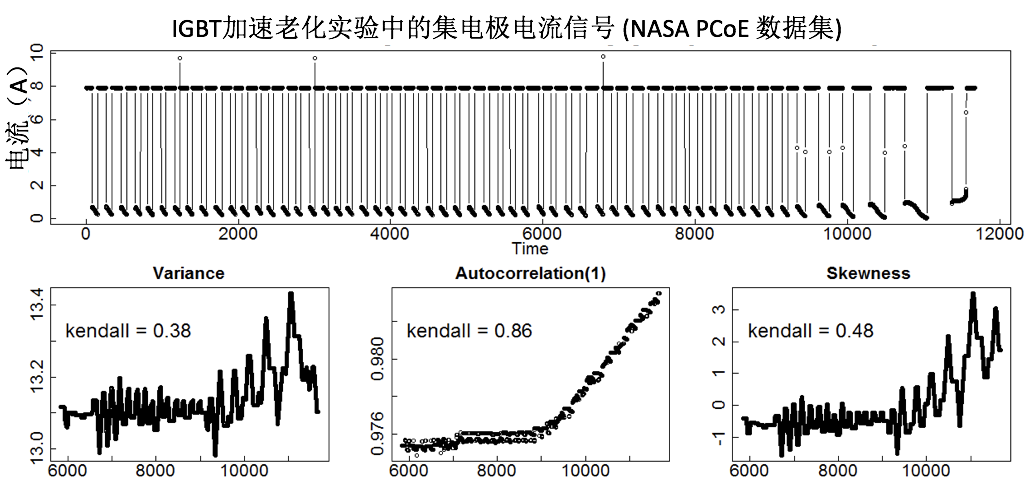
\includegraphics[scale=0.6]{figures/csd/csd-signal-igbt.png}
\end{subfigure}
\caption{基于各系统传感器信号学习的系统失效早期预警特征}
\label{fig:csd-early-signal}
\end{figure}

\begin{table}[htbp]
  \centering
  \caption{各系统早期预警特征的Mann-Kendall趋势指标}
  \label{tab:csd-kd-trend}
    \begin{tabular}{cccc}
      \toprule[1.5pt]
      {\heiti 系统/早期预警特征} & {\heiti Variance} & {\heiti Autocorrelation(1)}  & {\heiti Skewness}\\\midrule[1pt]
      柴油机车制动管 & 0.23 & 0.62 & 0.25 \\
      滚动轴承 & 0.50 & 0.40 & 0.56 \\
      涡轮发动机 & 0.64 & 0.82 & -0.55 \\ 
      IGBT & 0.38 & 0.86 & 0.48 \\
      \bottomrule[1.5pt]
    \end{tabular}
\end{table}

\begin{figure}[H]
\centering
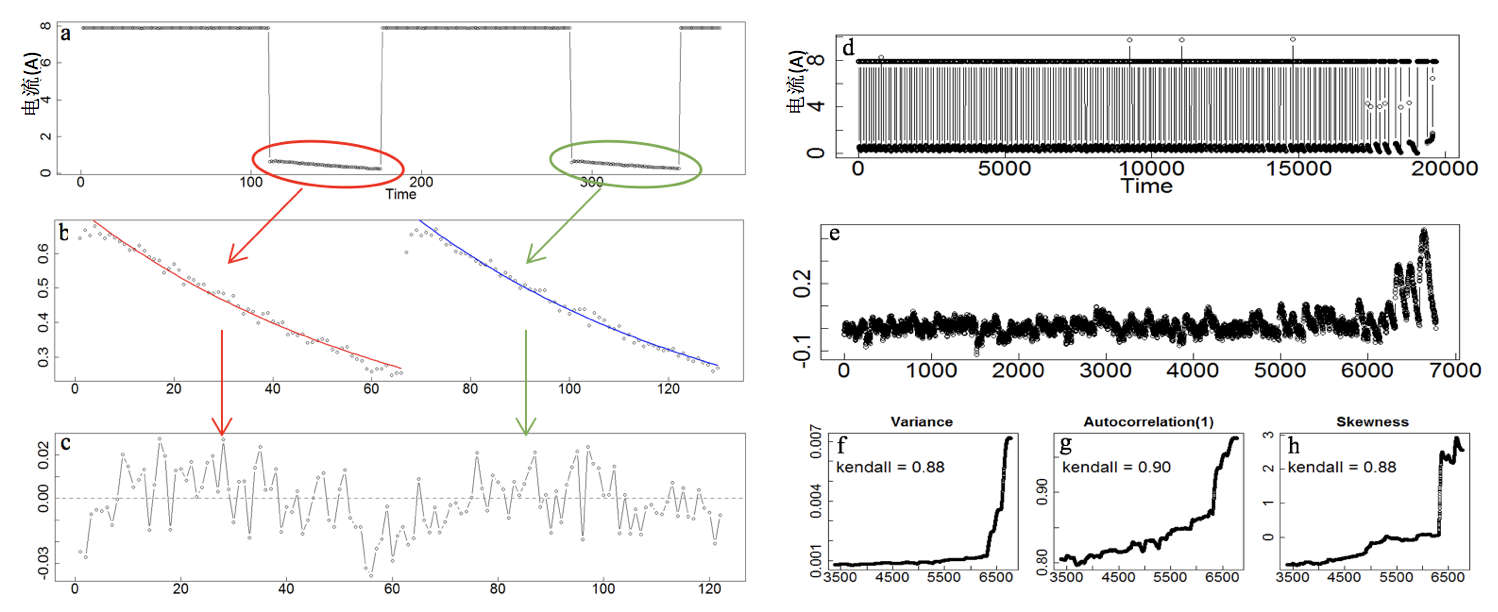
\includegraphics[scale=0.5]{figures/csd/fluctuation-mining.png}
\caption{以IGBT加速老化试验数据集为例的随机波动信号挖掘}
\label{fig:csd-fm-procedure}
\end{figure}

(3) 系统失效与临界相变的一致性检验结果展示

本文通过非参数的Wilcoxon检验方法、核密度估计检验方法、基于AIC的ARIMA模型分析以及动态系统稳定性分析,证明“系统失效引起系统状态转变”,进而将系统失效和临界相变关联起来。具体方法参见本章\ref{sec:csd-existence-test}。

\begin{figure}[H]
\centering
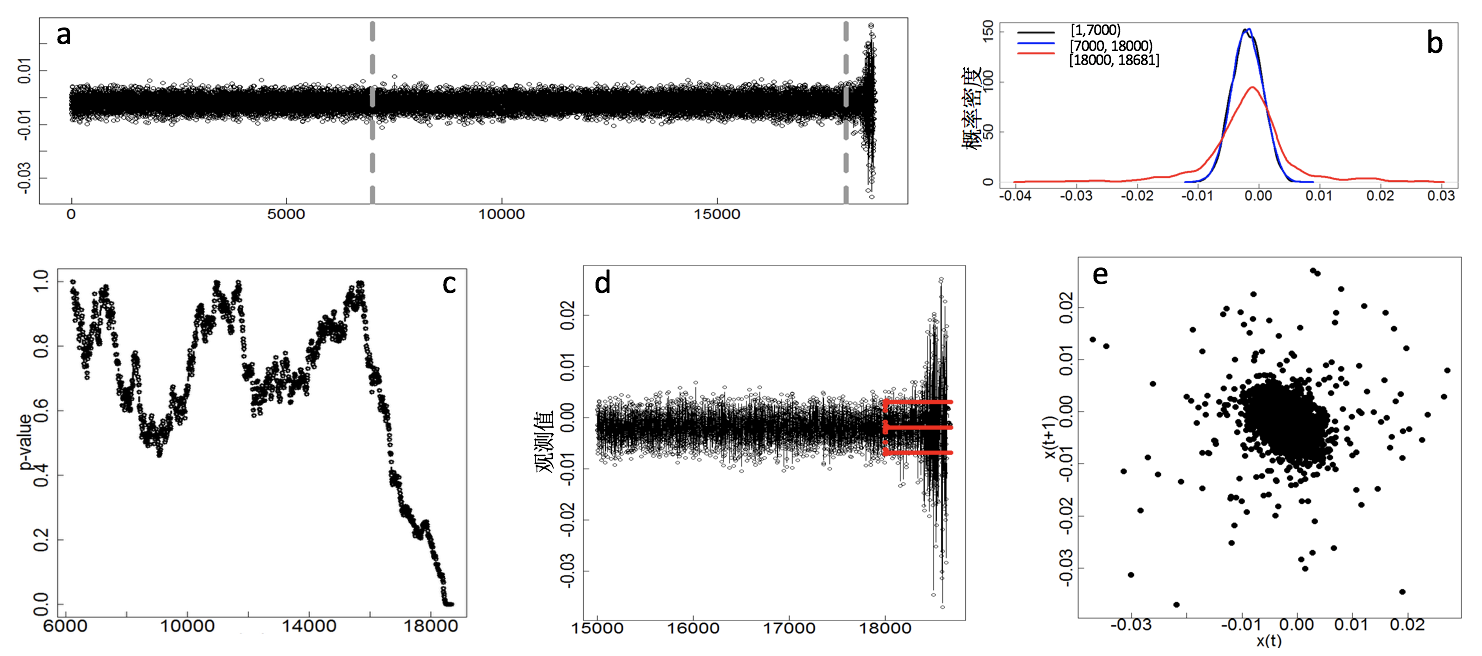
\includegraphics[scale=0.5]{figures/csd/csd-proof-bearing.png}
\caption{轴承系统失效与临界相变一致性检验结果}
\label{fig:csd-proof-bearing}
\end{figure}
针对滚动轴承系统的检验结果,如图\ref{fig:csd-proof-bearing}。\ref{fig:csd-proof-bearing}a 是原生时序震动信号,记为\emph{x},并将其分为不相交的三段,即$s1=x[1,6999], s2=x[7000,17999], s3=x[18000, 18681]$,其中$s1,s2$对应系统正常状态,而$s3$对应系统失效状态。由此展开以下4个方面的验证:

1. 基于高斯核的核密度估计检验结果,如图\ref{fig:csd-proof-bearing}b:$s1,s2$的概率密度趋于一致,而$s3$与前两者显著不同。

2. Wilcoxon检验结果,如图\ref{fig:csd-proof-bearing}c:将代表系统正常状态的$s1$固定,然后以大小为$w=6999$的滑窗从时刻7000开始往系统失效方向滑行,将每次获取的滑窗样本\emph{s}与$s1$进行Wilcoxon检验,并且原假设$H_{0}$为“两个被测样本服从同一分布”。检验结果表明,当滑窗到达时刻15000附近时$p$值急剧下降,当到达系统失效点时,$p$值低于0.01,有很强理由拒绝$H_{0}$,即可断定\emph{s}与$s1$源自不同分布。

3. 基于AIC的ARIMA模型分析的检验结果,如图\ref{fig:csd-proof-bearing}d:首先连接$s1,s2$得到对应系统正常状态的$s=x[1,17999]$,并以此作为训练数据集,基于AIC评估指标学习ARIMA模型;然后利用以上模型对$s3=x[18000, 18681]$进行预测,图示中红色区域是95\%置信度的预测区间;检验结果表明,预测区间可以包含正常状态的样本,但无法包含系统失效时发散的样本。

4. 基于动态系统稳定性分析的检验结果,如图\ref{fig:csd-proof-bearing}e:符号回归方法无法针对振动信号学习系统结构特征,因此采用离散系统下单变量的动态系统稳定性分析方法。首先,将一维振动信号映射到二维相空间以观察其运动轨迹,图中纵坐标为$x(t+1)$,横坐标为$x(t)$,因此图示实际是振动信号的一阶段差分,反映了动态系统的低阶运动轨迹。检验结果表明,$s1,s2$的运动收敛于固定点,而$s3$对应图中发散部分。

以上4个检验结果一致证明滚动轴承系统失效引起系统状态转变。

针对涡扇发动机系统的检验结果,如图\ref{fig:csd-proof}。将样本数据分成两段,$s1=[1,100]$对应系统正常状态,$s2=[101,192]	$对应系统从正常到失效的过程数据。通过符号回归方法学习$s1, s2$的微分方程。结果如\ref{fig:csd-proof}b所示,$s1$对应蓝色,运动方程收敛于固定点;$s2$对应红色曲线,有两个固定点,一个稳定点和一个非稳定点,系统运动具有不稳定性。检验结果证明涡扇发动机系统失效引起系统状态转变。

针对IGBT系统的检验结果,如图\ref{fig:csd-proof}。基于符号回归方法学习系统结构特征,又称吸引子。\ref{fig:csd-proof}c,d对应系统正常状态,系统运动过程中多个信号收敛于有限环。\ref{fig:csd-proof}e,f对应系统失效状态,系统运动过程中没有明显的收敛域。检验结果证明IGBT系统失效引起系统状态转变。


(4)针对早期预警特征的关键跳变检测算法实现故障预测的结果展示

通过本章\ref{sec:csd-application}提出的关键跳变检测算法确定系统失效早期预警特征的跳变点,置信水平$\alpha =0.05$,即置信度为95\%。柴油机车制动管、滚动轴承、涡扇发动机和IGBT的滑窗大小分别为2000,1000,20,1000。结果参见表\ref{tab:csd-alarm-time},早期预警特征的跳变点均早于系统失效时间,对潜在故障具有很好的预测能力。值得注意的是,为便于统一,此处的时刻代表相应数据集的样本编号。
%值得注意的是其中的时刻表示失效点或跳变点在时间序列中对应的下标二非具体的时间,具体的时间可通过采样率算出。比如采油机制动管的采样间隔为1s,分析时按10s进行重采样,早期预警指标比失效时间提前23000-18000=5000,那么实际的时间为10s*5000=50000s=13h,即早期预警指标可以提前13个小时预测到潜在故障。综上,临界相变早期预警指标在工程系统中的应用推广将为普适性的故障预测,PHM架构的部署开辟新的道路。
\begin{table}[htbp]
  \centering
  \caption{系统失效和早期预警特征的跳变时刻对比结果}
  \label{tab:csd-alarm-time}
    \begin{tabular}{ccc}
      \toprule[1.5pt]
      系统 & 失效时刻 &  早期预警特征跳变时刻  \\\midrule[1pt]
      柴油机车制动管 & 20747 & 18660 \\ 
      滚动轴承 & 18681 & 14302 \\
      涡扇发动机 & 192 & 149 \\
      IGBT & 11681 & 9184 \\
      \bottomrule[1.5pt]
    \end{tabular}
\end{table}
% Note: the first 1000 point of Bearing was discarded. 
% 窗口大小:
% 柴油机车制动管:2000
% 滚动轴承:1000
% 涡扇发动机:20
% IGBT:1000
\begin{figure}[H]
\centering
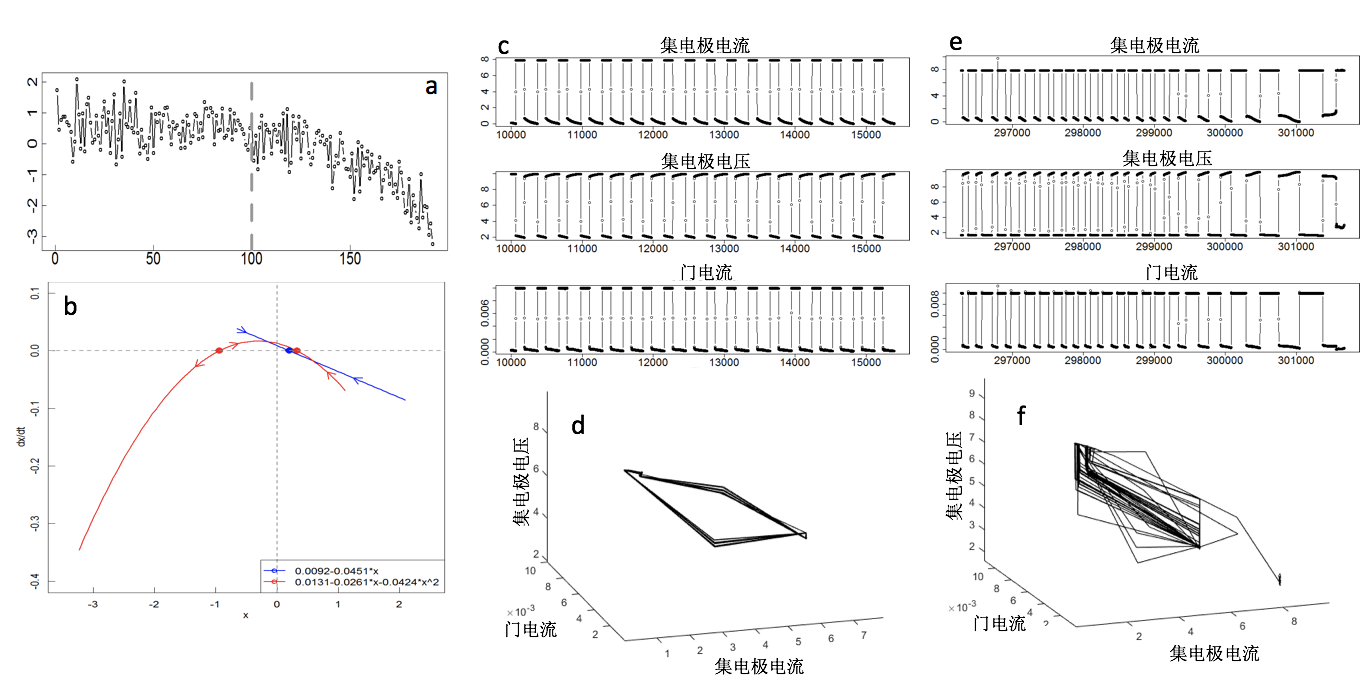
\includegraphics[scale=0.6]{figures/csd/csd-proof.png}
\caption{涡扇发动机和IGBT系统失效与临界相变一致性检验结果}
\label{fig:csd-proof}
\end{figure}

\section{小结}

本章首先对临界相变预测理论以及其与工业系统失效预测的契合点进行了论述;然后将复杂系统临界相变预测理论引入并提出针对工业系统失效预测的早期预警特征学习方法,通过4个不同类型的数据集展开研究。实验结果表明,本文方法可以从差异显著的工业时间序列数据中学习一致且显著的失效早期预警特征;通过多种方法验证了系统失效确实引起系统状态的急剧转变,进一步证明临界相变理论的适用性。最后针对早期预警特征,提出了关键跳变检测算法实现故障预测,实验结果表明早期预警特征跳变时间均显著早于系统失效时间,对潜在故障具有很好的预测能力。
